\documentclass[a4paper,11pt,parskip=half,headings=small,DIV=11,notitlepage,abstract=on]{scrartcl}
% This file contains configuration shared between main file and figures

\usepackage{pifont}
\usepackage{xspace}
\DeclareUnicodeCharacter{2460}{\ding{172}\xspace}
\DeclareUnicodeCharacter{2461}{\ding{173}\xspace}

\usepackage{tikz}

\definecolor{HB9UFblue}{RGB}{0,61,165}
\definecolor{HB9UFred}{HTML}{ED135A}

\newcommand{\Ohm}{$\Omega$\xspace}


\newcommand{\uline}[1]{%
  \tikz[baseline=(todotted.base)]{
      \node[inner sep=1pt,outer sep=0pt] (todotted) {#1};
      \draw[color=HB9UFblue,thick] (todotted.south west) -- (todotted.south east);
  }%
}%
                           
\newcommand{\udash}[1]{%
  \tikz[baseline=(todotted.base)]{
      \node[inner sep=1pt,outer sep=0pt] (todotted) {#1};
      \draw[dashed,color=HB9UFred,thick] (todotted.south west) -- (todotted.south east);
  }%
}%

\usepackage{scrlayer-scrpage}
\usepackage{graphicx}
\usepackage{amsmath}
\usepackage[pdfauthor={},pdftitle={},pdfstartview=FitH,pdfborder={0 0 0}]{hyperref}
\usepackage[utf8]{inputenc}
\usepackage{textcomp}
\renewcommand{\thesection}{\Alph{section}}
\renewcommand*{\theenumi}{\thesection.\arabic{enumi}}

\usepackage{ngerman}
\ifoot{\texttt{}}
\ofoot{\texttt{}}

%\addtolength{\textheight}{5mm}
\title{Posten A\\ Reflexionsmessungen passiver Bauteile}
\author{}
\date{}
\pagestyle{empty}
\renewcommand*{\titlepagestyle}{empty}
\sloppy

\begin{document}
\maketitle
\vspace{-2cm}

An diesem Posten bestimmst du Wirk- und Blindwiderstand, Kapazität bzw. Induktivität von passiven Bauteilen wie Widerstand, Spulen und Kondensatoren. Es gibt für diese Messung verschiedene Varianten, die in Kapital 4 des NanoVNA Primers aufgezeigt werden. Wir wählen an dieser Stelle eine einfache Reflexionsmessung, so dass die Bauteile folgendermassen mit dem NanoVNA verbunden werden:

\begin{center}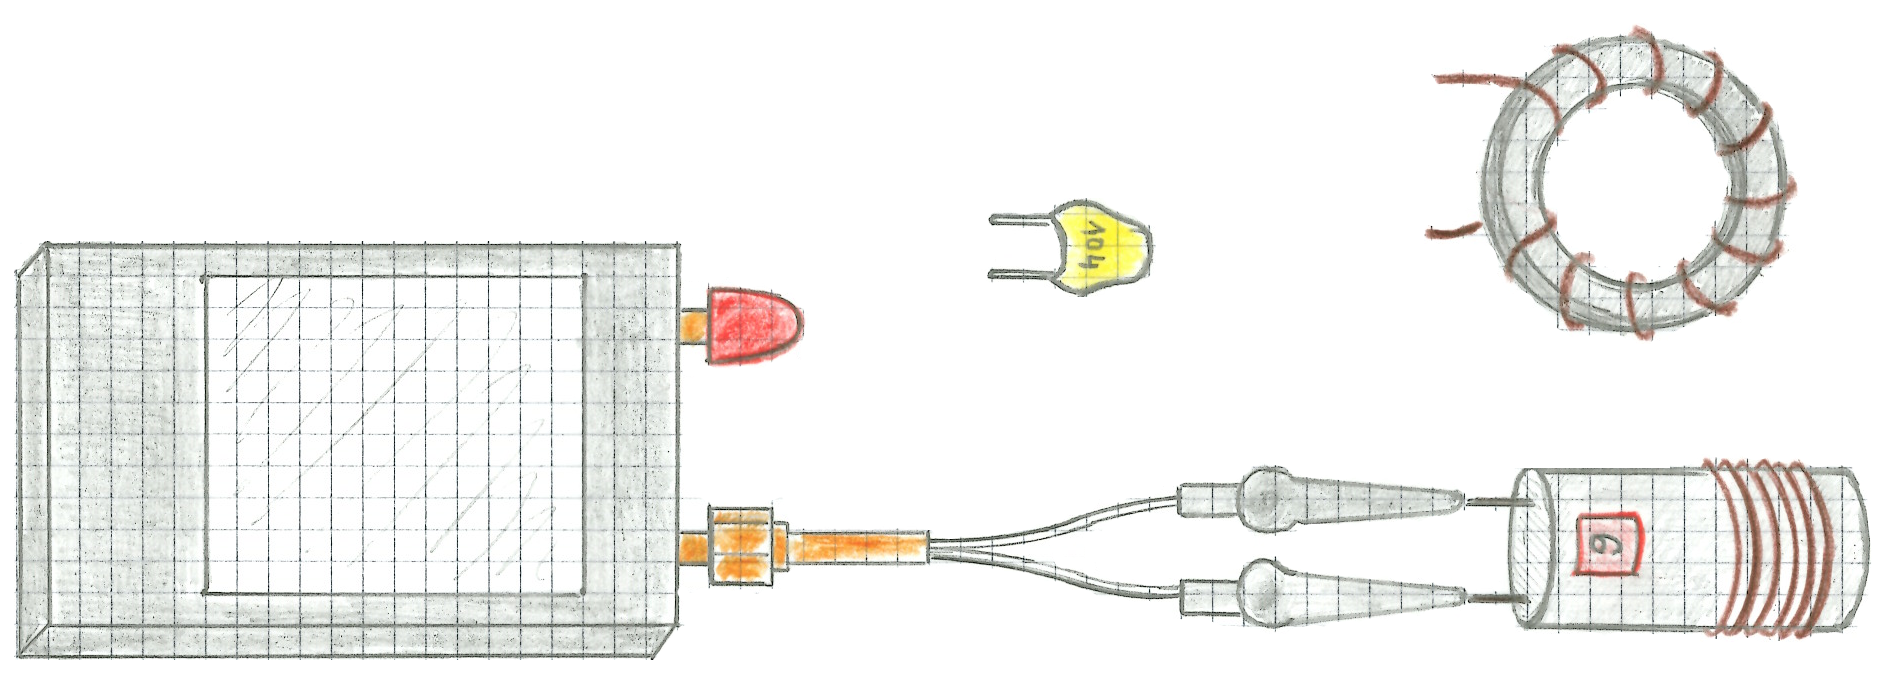
\includegraphics[width=.65\textwidth]{../skript/figures/illustration_impedance.png}\end{center}

Für die Berechnung von Stehwellenverhältnis (SWR), induktivem Blindwiderstand ($X_L$) und kapazitivem Blindwiderstand ($X_C$) sind die Formeln
\begin{align*}
    \text{SWR} &= \max\left\{\frac{Z_0}{R}, \frac{R}{Z_0}\right\} & X_L &= 2\pi f L & X_C &= \frac{1}{2\pi f C}
\end{align*}
relevant, wobei $f$ die Frequenz, $Z_0$ die System-Impedanz, $R$ der Widerstand, $L$ die Induktivität und $C$ die Kapazität des Prüflings ist.

Aus diesen Formeln ergeben sich folgende Aussagen:
\begin{itemize}
    \item In einem $50$~\Ohm-System haben eine 100~\Ohm-Last und eine 25~\Ohm-Last beide jeweils ein SWR von 2; eine 50~\Ohm-Last hat eine SWR von 1.
    \item Der Blindwiderstand einer idealen Spule nimmt mit der Frequenz zu.
    \item Der Blindwiderstand eines idealen Kondensators nimmt mit der Frequenz ab.
\end{itemize}
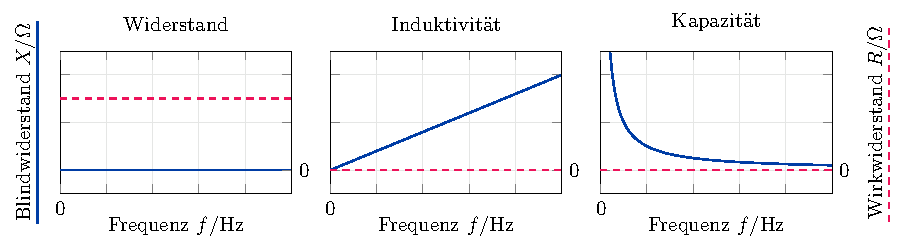
\includegraphics[width=\textwidth]{../skript/figures/reactance/reactance.pdf}

\section{Messung von Widerständen}
\begin{enumerate}
    \item Wähle einen Frequenzbereich von 1~MHz bis 30~MHz und kalibriere den VNA für eine Reflexionsmessung.
    \item Wähle im Display-Menü ein Trace-Format von \textbf{``Resistance''}. Damit wird der Wirkwiderstand angezeigt.
    \item Notiere den Widerstand der folgenden Schaltungen aus 100~\Ohm-Widerständen:
        \begin{enumerate}
            \item Ein 100~\Ohm-Widerstand.
            \item Zwei in Serie geschaltete 100~\Ohm-Widerstände.
            \item Zwei parallel geschaltete 100~\Ohm-Widerstände.
        \end{enumerate}
    \item Wähle nun ein Trace-Format von \textbf{``SWR''} und wiederhole deine Messung. Beurteile das Resultat.
\end{enumerate}

\section{Messung einzelner Induktivitäten und Kapazitäten}
\begin{enumerate}
    \item Wähle einen Frequenzbereich von 1~MHz bis 30~MHz und kalibriere den VNA für eine Reflexionsmessung.
    \item Wähle im Display-Menü ein Trace-Format von \textbf{``Reactance''}. Damit wird der Blindwiderstand angezeigt.
    \item Es liegen verschiedene Spulen und Kondensatoren zum Ausmessen aus (1~\textmu H, 100~pF, 470~pF). Miss den Blindwiderstand und vergleiche mit der Theorie.
    \item Wähle nun ein Trace-Format von \textbf{``Series L''} bzw. \textbf{``Series C''} und wiederhole deine Messung. Was fällt auf?
    \item Wiederhole die Messung des Blindwiderstandes der Spule in einem erweiterten Frequenzbereich. Setze dazu den Stimulus auf eine Stop-Frequenz von 250~MHz und rekalibriere das Gerät. Was stellst du fest?
    \item Bei welcher Frequenz hat die 1~\textmu H-Spule einen Blindwiderstand von 100~\Ohm? Dieser Widerstand in einem 50~\Ohm würde einem
        SWR von 2 entsprechen. Prüfe diese Hypothese mit einer Messung und überlege dir, weshalb sie falsch ist.
\end{enumerate}

\section{Schwingkreis}
\begin{enumerate}
    \item Wähle einen Frequenzbereich von 1~MHz bis 30~MHz und kalibriere den VNA für eine Reflexionsmessung.
    \item Miss zunächst die einzelnen Elemente des Serienschwingkreises aus.
    \item Bestimme Wirk- und Blindwiderstand des gesamten Schwingkreises und dessen SWR. Auf welcher Frequenz ist der Schwingkreis resonant?
\end{enumerate}
\end{document}
